% Zeilenabstand 1,5 Zeilen -----------------------------------------------------
\onehalfspacing

% Seitenr�nder -----------------------------------------------------------------
\setlength{\topskip}{\ht\strutbox} % behebt Warnung von geometry
\geometry{paper=a4paper,left=30mm,right=30mm,top=30mm}

% Kopf- und Fu�zeilen ----------------------------------------------------------
\pagestyle{scrheadings}
% Kopf- und Fu�zeile auch auf Kapitelanfangsseiten
\renewcommand*{\chapterpagestyle}{scrheadings} 
% Schriftform der Kopfzeile
\renewcommand{\headfont}{\normalfont}

% Kopfzeile alt mit fehler
%\ihead{
%%\large{\textsc{\titel}}\\ \small{\untertitel} \\[2ex] 
%\textit{\headmark}}
%\chead{}
%%\ohead{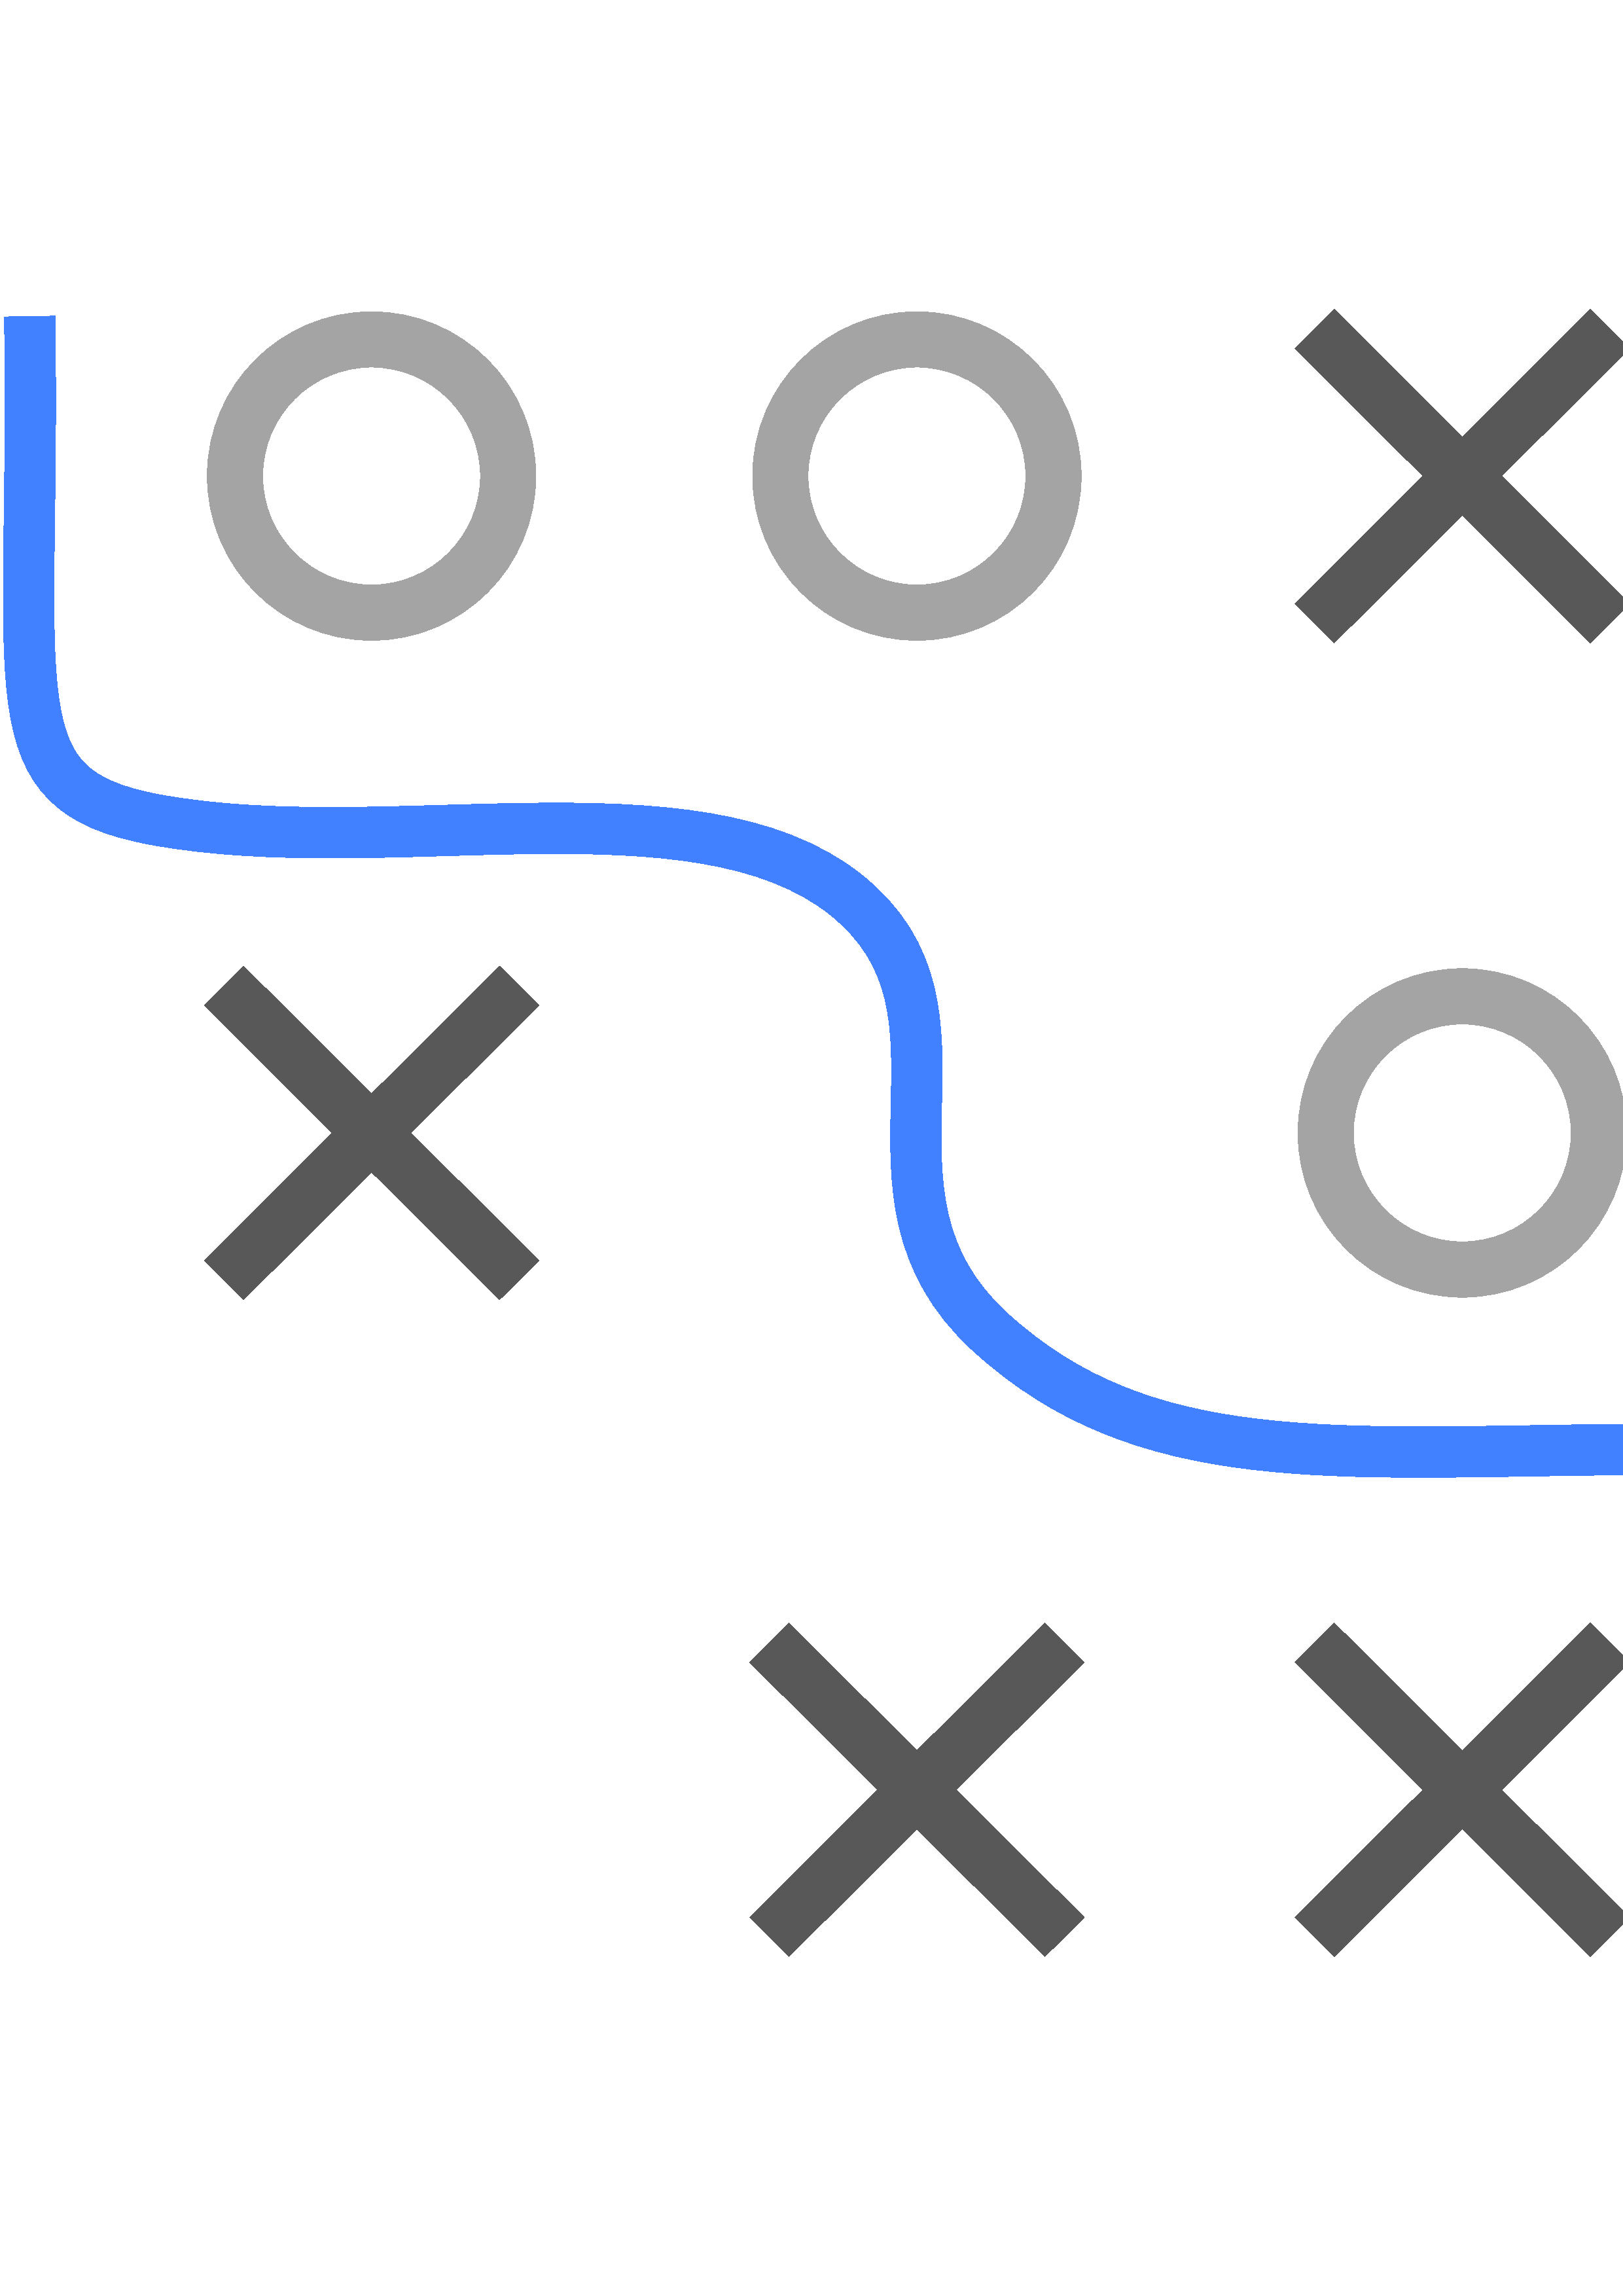
\includegraphics[scale=0.15]{\logo}}
%\setlength{\headheight}{21mm} % H�he der Kopfzeile
%% Kopfzeile �ber den Text hinaus verbreitern
%\setheadwidth[0pt]{textwithmarginpar} 
%\setheadsepline[text]{0.4pt} % Trennlinie unter Kopfzeile


% Kopfzeile
%\ihead{\textit{\headmark}}
%\chead{}
%\setlength{\headheight}{21mm} % H�he der Kopfzeile
% Kopfzeile �ber den Text hinaus verbreitern
%\setheadwidth[0pt]{textwithmarginpar} 
%\setheadsepline[text]{0.4pt} % Trennlinie unter Kopfzeile



% Fu�zeile
%\ifoot{\copyright\ \autor}
%\cfoot{}
%\ofoot{\pagemark}

% sonstige typographische Einstellungen ----------------------------------------

% erzeugt ein wenig mehr Platz hinter einem Punkt
\frenchspacing 

% Schusterjungen und Hurenkinder vermeiden
\clubpenalty = 10000
\widowpenalty = 10000 
\displaywidowpenalty = 10000

% Quellcode-Ausgabe formatieren
\lstset{numbers=left, numberstyle=\tiny, numbersep=5pt, breaklines=true}
\lstset{emph={square}, emphstyle=\color{red}, emph={[2]root,base}, emphstyle={[2]\color{blue}}}

% Fu�noten fortlaufend durchnummerieren
%\counterwithout{footnote}{chapter}
